\documentclass[aspectratio=169]{beamer}
\usepackage{listings}
\usepackage{tikz}
\usetikzlibrary{shapes,shapes.multipart,arrows,positioning}

\beamertemplatenavigationsymbolsempty

\lstset{
  basicstyle=\ttfamily,
}

\newcommand{\filename}[1]{\texttt{#1}}
\newcommand{\dirname}[1]{\texttt{#1/}}
\newcommand{\command}[1]{\texttt{#1}}
\newcommand{\variable}[1]{\textit{#1}}
\newcommand{\branchname}[1]{\texttt{#1}}

\title{Schema Inference on Wikidata}
\subtitle{Final presentation}
\author{Lucas Werkmeister}
\date{2019-02-20}

\begin{document}

\frame{\titlepage}

\begin{frame}
  \frametitle{Wikidata}
  \begin{figure}
    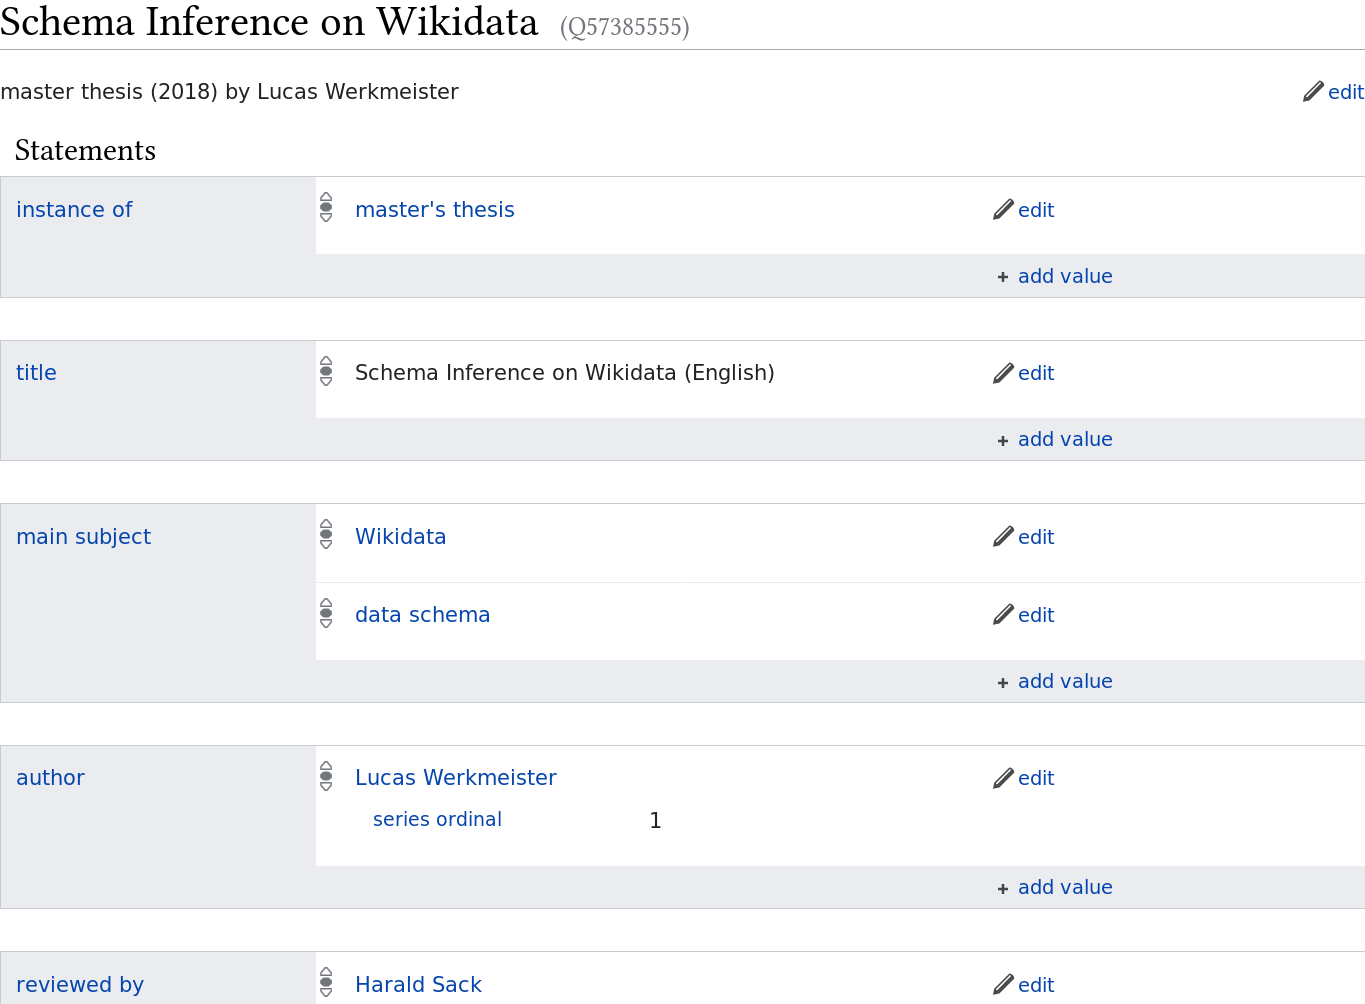
\includegraphics[width=0.7\textwidth]{item}
  \end{figure}
\end{frame}

\begin{frame}
  \frametitle{Wikidata}
  \begin{figure}
    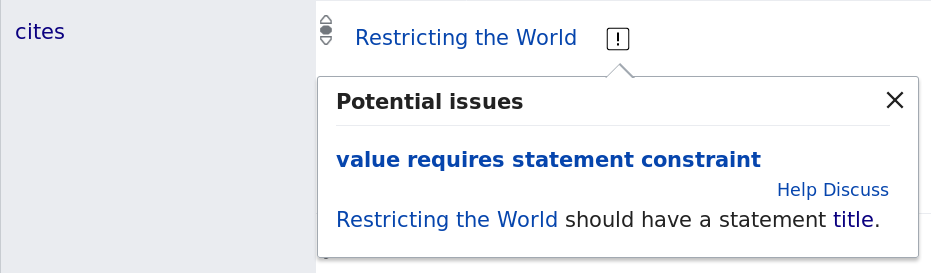
\includegraphics[width=0.8\textwidth]{constraint}
  \end{figure}
\end{frame}

\begin{frame}[fragile]
  \frametitle{Shape Expressions (ShEx)}
  \begin{figure}
    \begin{lstlisting}[language=sparql]
<master_thesis> {
  wdt:P1476 xsd:langString; # title
  wdt:P50 @<human>+ # author
}

<human> {
  wdt:P569 xsd:dateTime; # date of birth
  wdt:P570 xsd:dateTime? # date of death
}
    \end{lstlisting}
  \end{figure}
\end{frame}

\begin{frame}
  \frametitle{RDF2Graph}
  \vspace{-5cm}
  \begin{figure}
    \centering
    % TODO horizontal zig-zag instead of 50% scale?
    \begin{tikzpicture}[transform canvas={scale=0.5}]
      \tikzstyle{file} = [rectangle, draw, rounded corners, text centered]
      \tikzstyle{pipe} = [style=file, dashed]
      \tikzstyle{directory} = [rectangle, draw, text centered]
      \tikzstyle{arrow} = [draw, -latex', right]

      \begin{scope}[node distance=2cm]
        \node[file] (entities) {\filename{\variable{example}.entities.sparql}};
        \node[file, below of=entities] (data) {\filename{\variable{example}.data.sparql}};
        \node[pipe, below of=data] (JSON) {\filename{\variable{example}.json}};
        \node[file, below of=JSON] (N-Triples) {\filename{\variable{example}.nt}};
        \node[directory, below of=N-Triples] (Fuseki) [align=center] {\dirname{\variable{example}-fuseki} \\ \texttt{http://localhost:3030/\variable{example}/query}};
        \node[directory, below of=Fuseki] (RDF2Graph) {\dirname{\variable{example}-results}};
        \node[file, below of=RDF2Graph] (ShEx) {\filename{\variable{example}.shex}};
        \node[file, below of=ShEx] (HTML) {\filename{\variable{example}.html}};
      \end{scope}

      \begin{scope}[every path/.style=arrow, midway]
        \path (entities) -- node {\command{sed}} (data);
        \path (data) -- node {WDQS} (JSON);
        \path (JSON) -- node {\command{jq}} (N-Triples);
        \path (N-Triples) -- node {Fuseki} (Fuseki);
        \path (Fuseki) -- node {RDF2Graph} (RDF2Graph);
        \path [dashed] (RDF2Graph.north east) to [out=30,in=330,looseness=5] node {RDF2Graph, simplify} (RDF2Graph.south east);
        \path (RDF2Graph) -- node {ShEx exporter} (ShEx);
        \path (ShEx) -- node {\command{pygmentize}} (HTML);
      \end{scope}
    \end{tikzpicture}
  \end{figure}
\end{frame}

\begin{frame}
  \frametitle{Adjustments, updates and fixes}
  \begin{itemize}
  \item adjust type predicates
  \item data download step
  \item reduce input data
  \item make simplification less aggressive
  \item support cycles in simplification
  \end{itemize}
\end{frame}

\begin{frame}
  \frametitle{Wikidata Shape Expressions Inference Tool}
  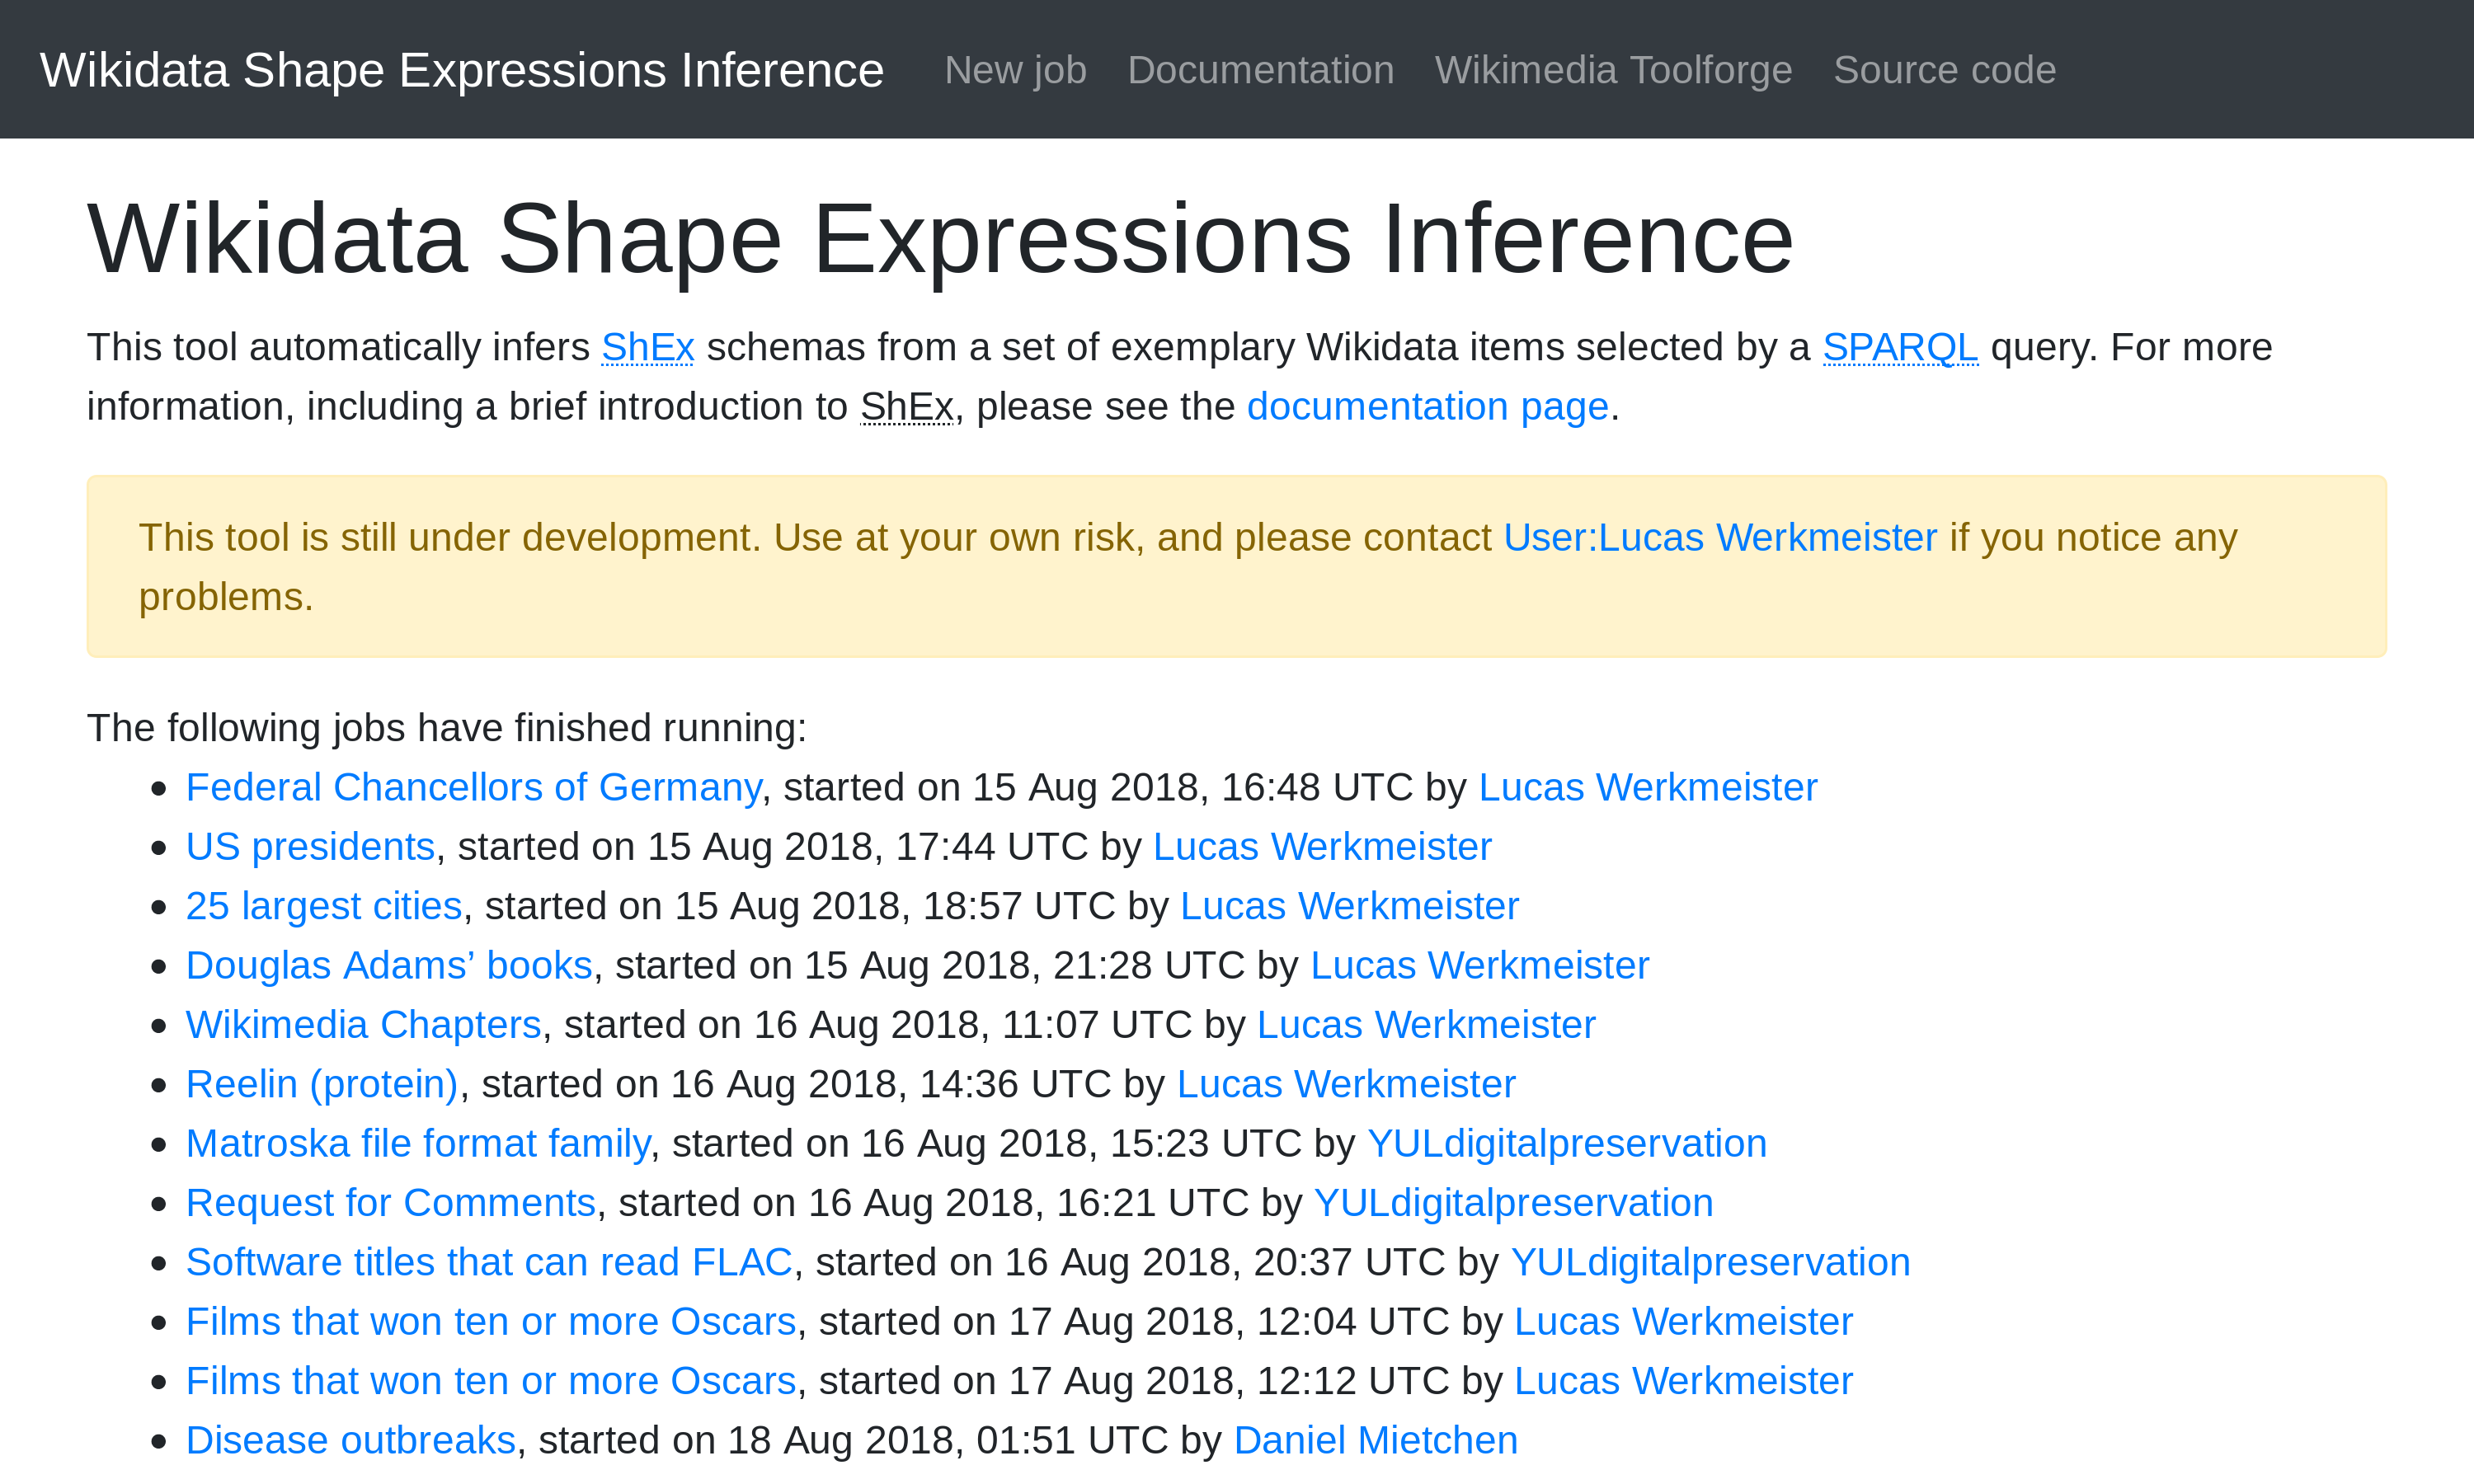
\includegraphics[width=\textwidth]{../screenshots/wdsi-index}
\end{frame}

\begin{frame}
  \frametitle{Wikidata Shape Expressions Inference Tool}
  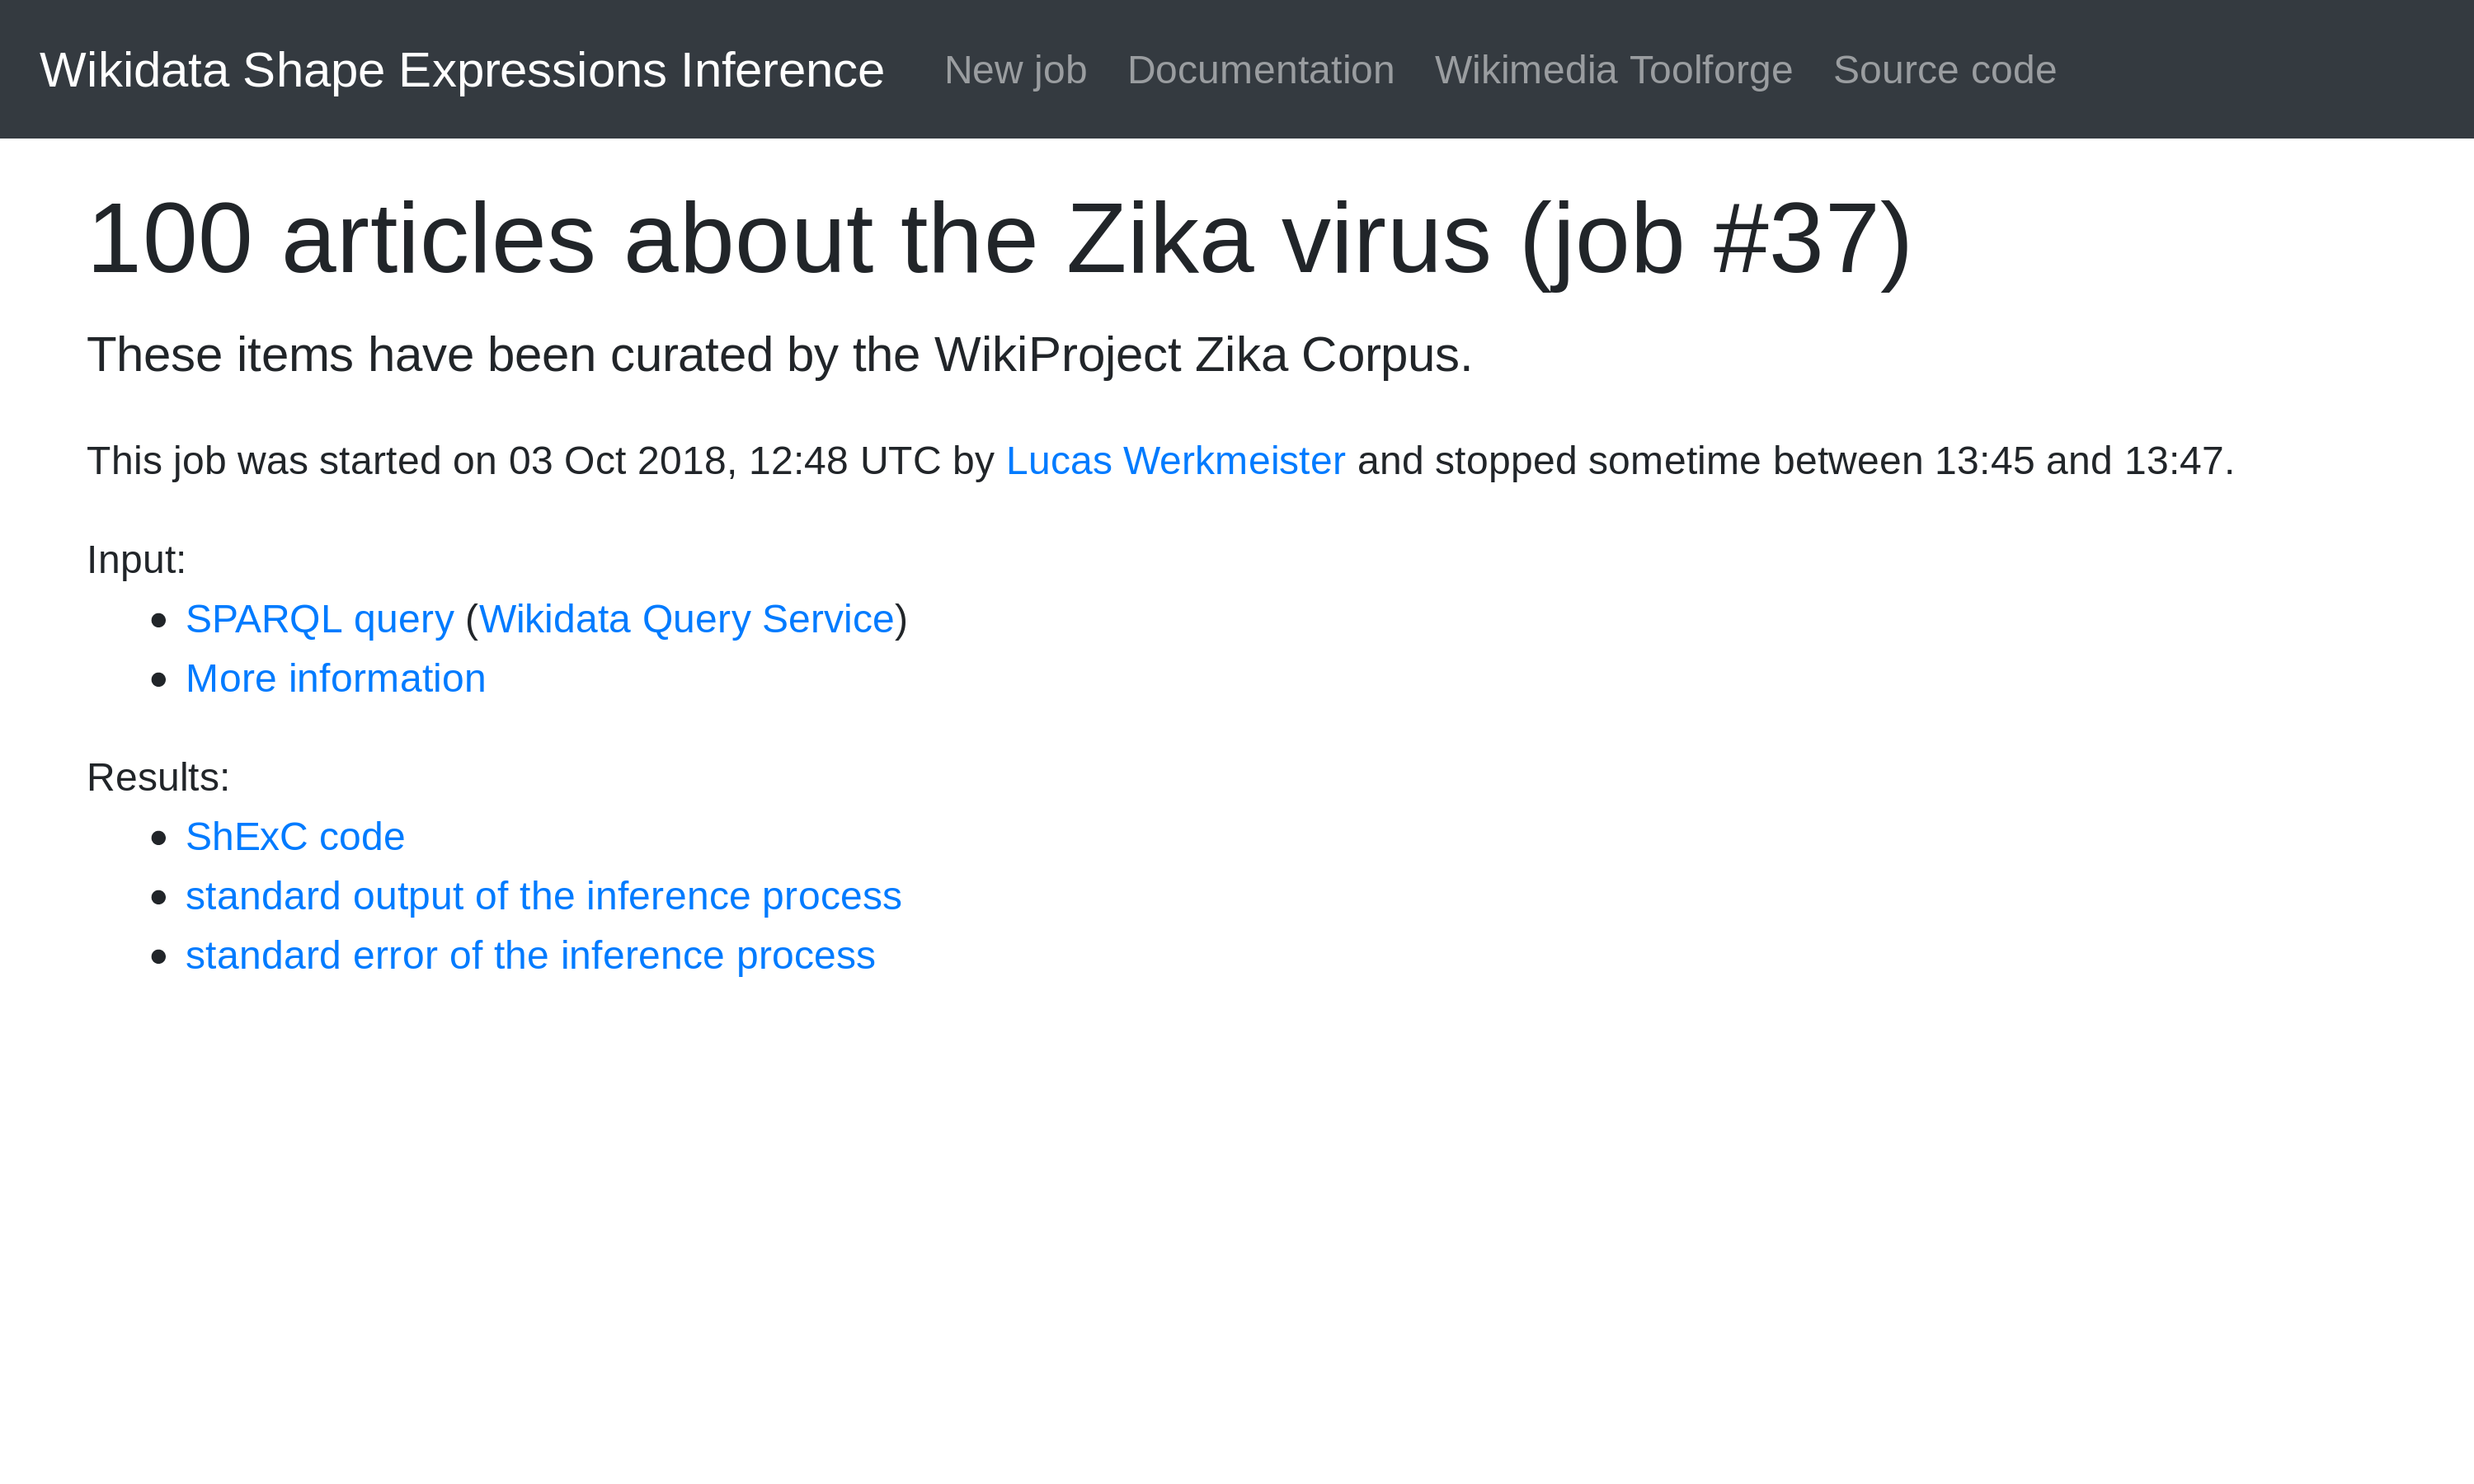
\includegraphics[width=\textwidth]{../screenshots/wdsi-zika}
\end{frame}

\begin{frame}
  \frametitle{Validation problems}
  \begin{itemize}
  \item reduce schemas on export
  \item depth limit in validator
  \end{itemize}
\end{frame}

\begin{frame}
  \frametitle{Resulting schemas}
  \begin{itemize}
  \item problems in schema can highlight problems in input data
  \item inferred schemas useful as basis for manually extracted ones
  \end{itemize}
\end{frame}

\begin{frame}
  \frametitle{Outlook}
  \begin{itemize}
  \item submit RDF2Graph improvements upstream
  \item tool improvements
  \item optimizations
  \item ShEx+Wikidata integration
  \end{itemize}
\end{frame}

\begin{frame}
  \frametitle{Thanks for your attention!}
  \begin{itemize}
  \item thesis with source code: \url{https://github.com/lucaswerkmeister/master-thesis}
  \item tool: \url{https://tools.wmflabs.org/wd-shex-infer/}
  \item questions / contact: \href{mailto:mail@lucaswerkmeister.de}{mail@lucaswerkmeister.de}
  \end{itemize}
\end{frame}

\end{document}
